\documentclass[12pt, a4paper]{article}
\usepackage{array}
\usepackage{longtable}
\usepackage[table]{xcolor}
\usepackage{hyperref}
\usepackage{float}
\usepackage[utf8]{inputenc}
\usepackage{graphicx}
\usepackage{amsmath}
\usepackage[margin=1 in]{geometry}
\usepackage{color}
\usepackage{caption}
\usepackage{pdflscape}
\usepackage{fancyhdr}

\title{Assignment 1: Foundations\\Statistical Methods for Machine Learning}
\author{Troels Thomsen - qvw203\\Rasmus Haarslev - nkh877\\Allan Martin Nielsen - jcl187}

\setlength\parindent{0pt}		% noindent through whole document
\usepackage[parfill]{parskip}	% extra linebreak on new paragraph

\begin{document}
\pagestyle{empty}
\maketitle
\newpage

\pagestyle{fancy}
\fancyhead[LO,LE]{qvw203 - nkh877 - jcl187}
\fancyhead[RO, RE]{Assignment 1}

\section{I.2.1}
\begin{itemize}
\item \textit{plot for $(\mu, \sigma) = {(-1, 1), (1, 2), (2, 3)}$}

\begin{figure}[!h]
    \centering
    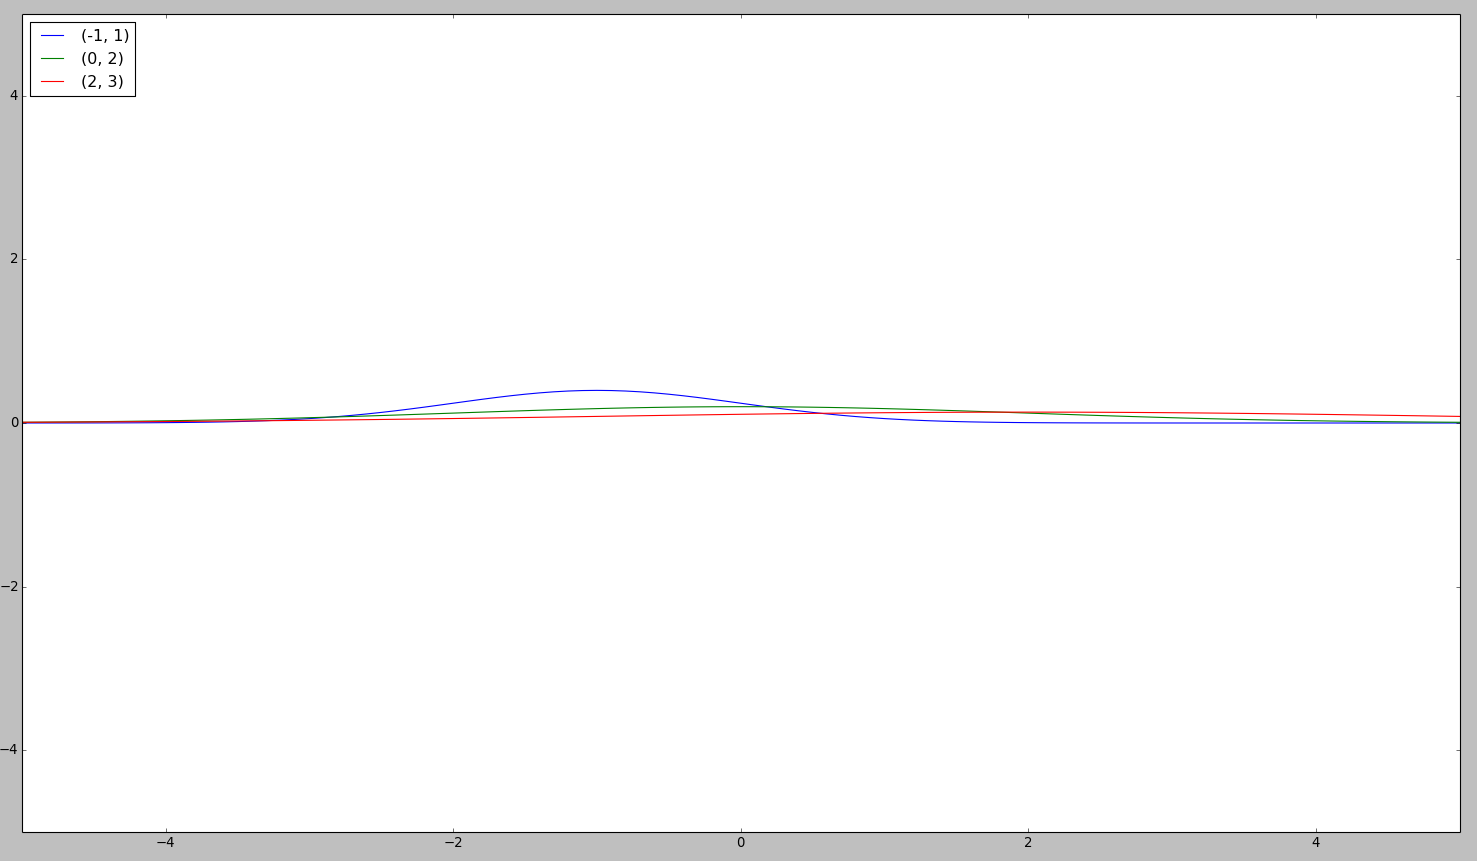
\includegraphics[width=0.9\textwidth]{1.png}
    \caption{$(\mu, \sigma)$}
    \label{fig:awesome_image}
\end{figure}
\end{itemize}
\section{I.2.2}
\begin{itemize}
\item \textit{Plot your dataset}

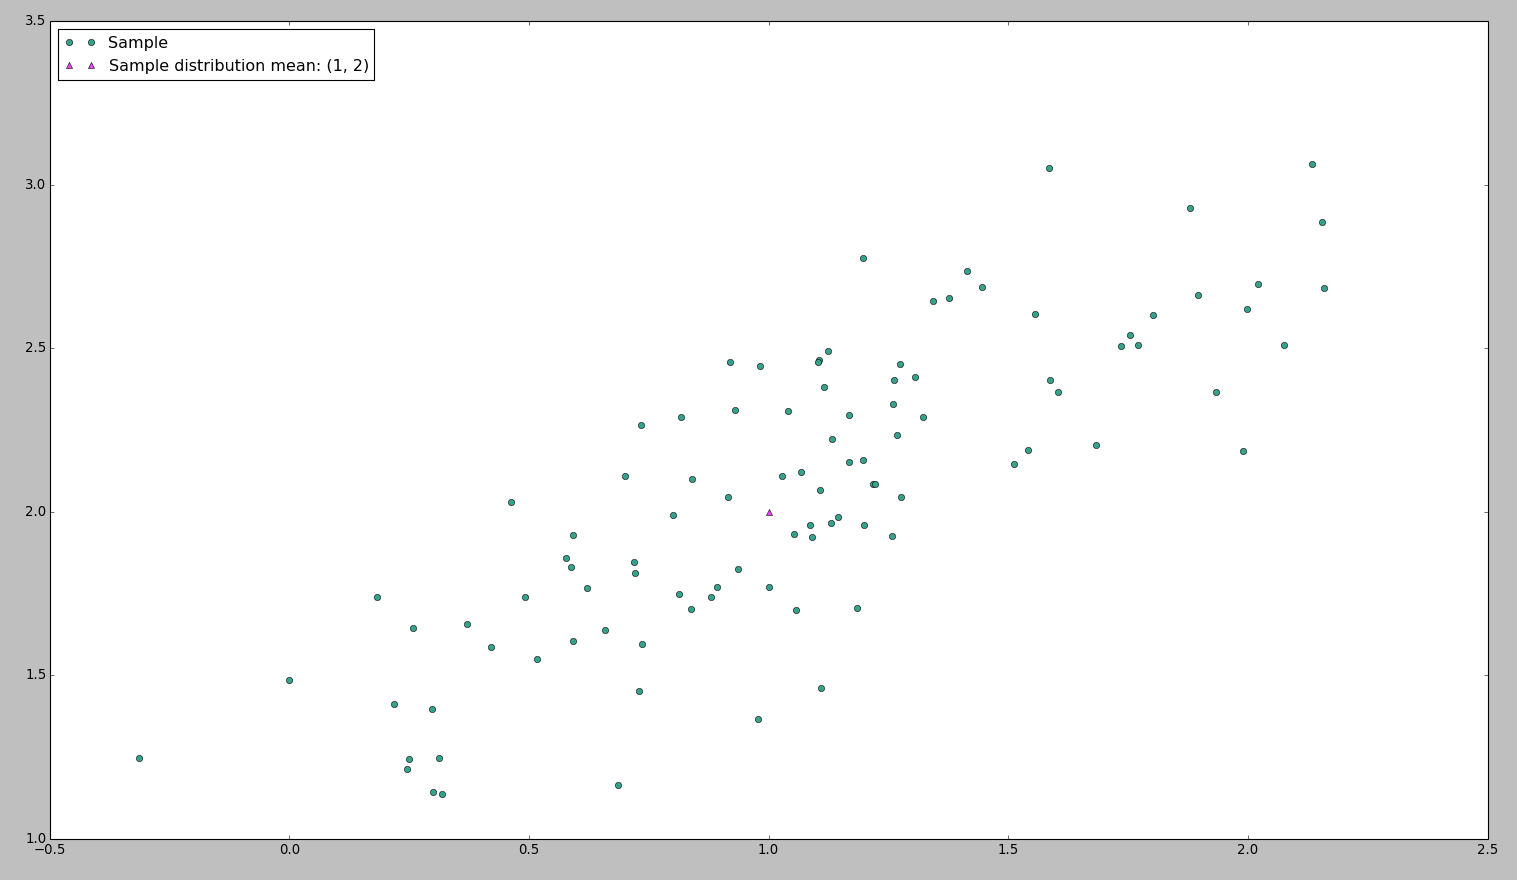
\includegraphics[width=0.9\textwidth]{2.png}

\end{itemize}

\section{I.2.3}
\begin{itemize}
\item \textit{Estimate the maximum likelihood sample mean of the data set}
\item \textit{Plot the sample mean and distribution mean as points in a 2-dimensional plot
together with the data points.}

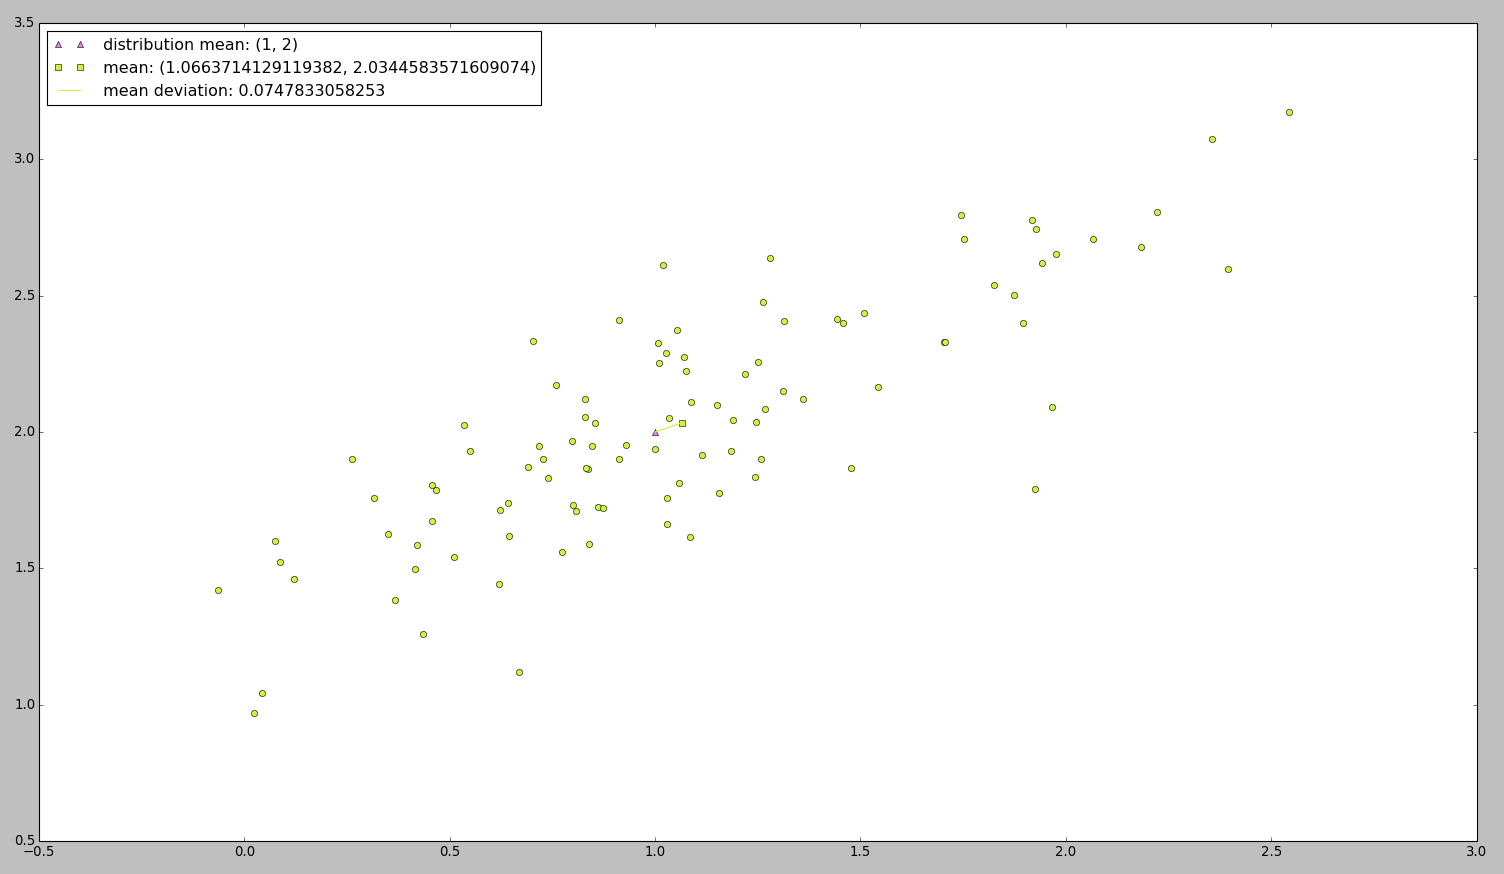
\includegraphics[width=\textwidth]{3.png}

\item Quantify how much the sample mean deviate from
the distribution mean.
\item Why do you see a deviation from the distribution mean (concis diskussion)
\end{itemize}



\section{I.2.4}
\begin{itemize}
\item \textit{Plot the scaled and translated eigenvectors
$\mu + \sqrt{\lambda_i} * e_i$}

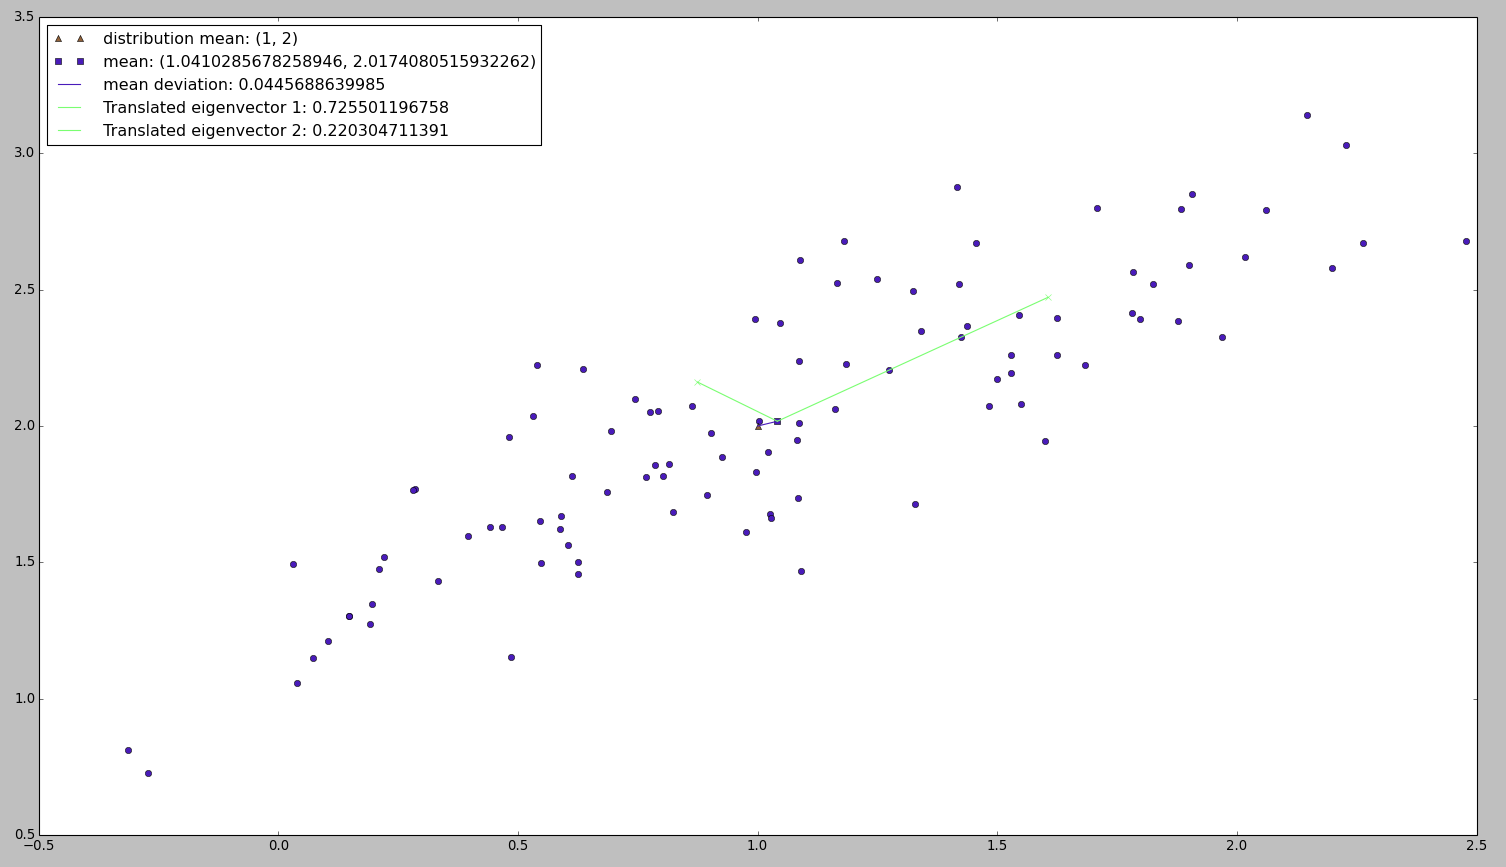
\includegraphics[width=\textwidth]{5.png}

\item \textit{Discuss how to interpret the
eigenvectors and eigenvalues of $\sum _{ML} $
on top of the sampled data from Question I.2.2}

The length of the scaled and translated eigenvectors represent the spread from the sample mean in orthogonal directions. 

\item \textit{Plot the samples from the rotated distributions in different colors in a combined plot.}

Underneath is a figure showing the original and the three rotated distributions, all in different colors.

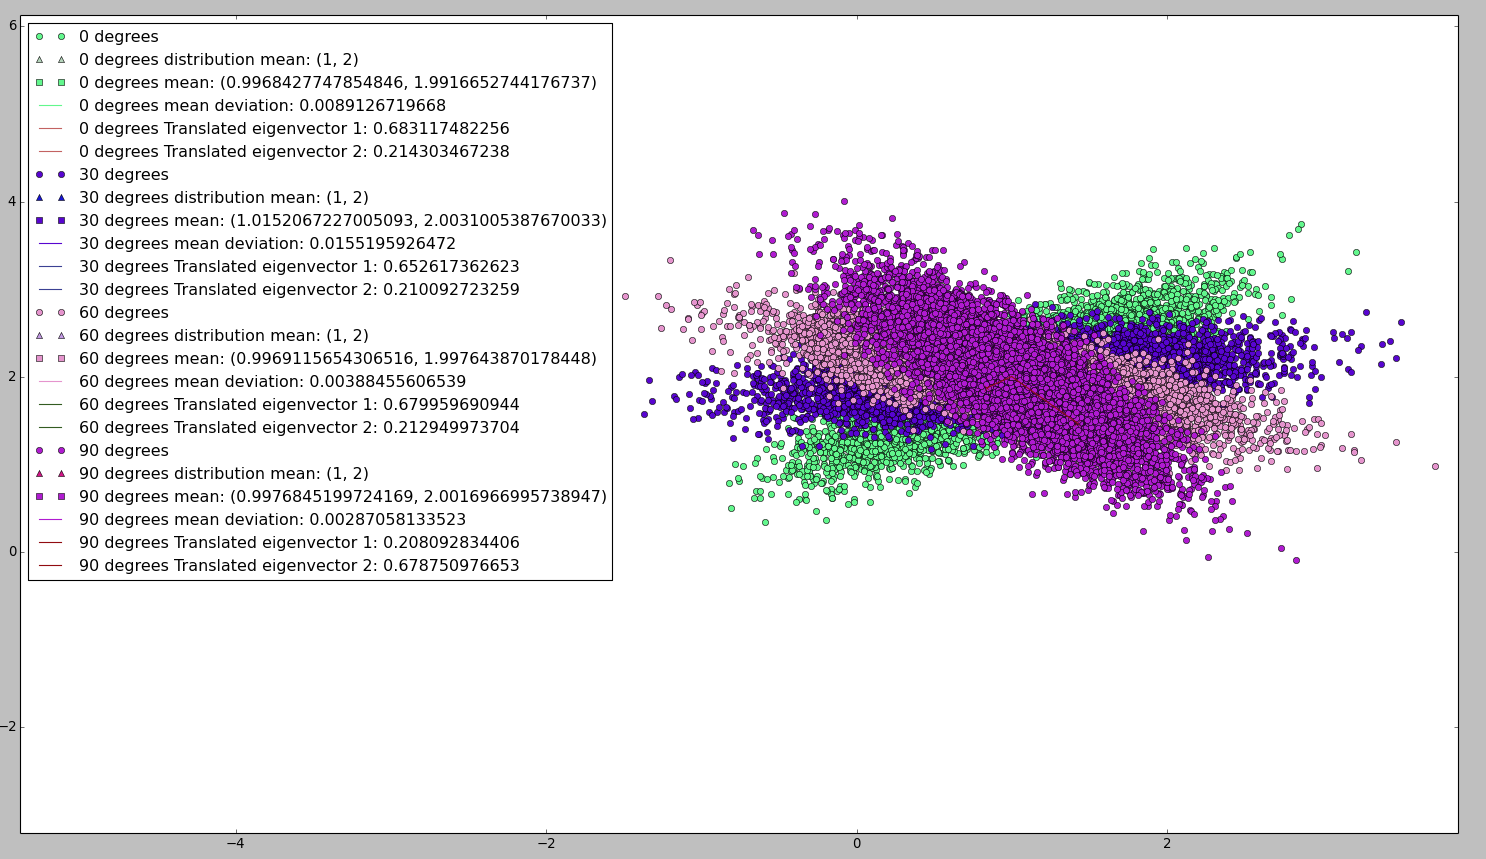
\includegraphics[width=\textwidth]{6.png}

\item \textit{Explain what you see.}

We see that the distributions are rotated their respective angles around the distribution mean.

\item \textit{Can you find an angle $\phi$ such that the main direction of the data sampled from the Gaussian distribution $\mathcal{N}(y|\mu, \sum \phi )$ points along the x axis?}

To find this angle we use the information, that when it is rotated this way, the eigenvector describing the width of the spread, will be orthogonal on the x-axis and therefore directly vertical (its x-direction is zero and its y-direction is exactly its length).

\item \textit{Can you find an angle $\phi$ such that the main direction of the data sampled from the Gaussian distribution $\mathcal{N}(y|\mu, \sum \phi )$ points along the x axis?}

To find this angle we use the information, that when it is rotated this way, the eigenvector describing the width of the spread, will be orthogonal on the x-axis and therefore directly vertical (its x-direction is zero and its y-direction is exactly its length).

Knowing this, we can isolate $\phi$ in the equation for rotating a vector. It will still have the same length as before, so we can set up the following equation, where \textbf{a} is the vector to be rotated and \textbf{R} is the rotation-matrix:
\begin{equation*}
\left( \begin{array}{c}
0 \\
|\textbf{a}| \end{array} \right)
=
\textbf{R}\textbf{a}
\end{equation*}
\begin{equation*}
\left( \begin{array}{c}
0 \\
\sqrt{x_a^2+y_a^2} 
\end{array} \right)
=
\left( \begin{array}{cc}
\cos \phi & -\sin \phi \\
\sin \phi & \cos \phi \end{array} \right)
\left( \begin{array}{c}
x_a \\
y_a \end{array} \right)
\end{equation*} 
Now we can isolate $\phi$ and find a general equation for calculating this angle to align the length of the spread, with the x-axis:
\begin{equation*}
\phi = cos^{-1}\left(\dfrac{y_a}{\sqrt{x_a^2+y_a^2}}\right)
\end{equation*} 
Underneath is a figure showing the original and aligned distribution.

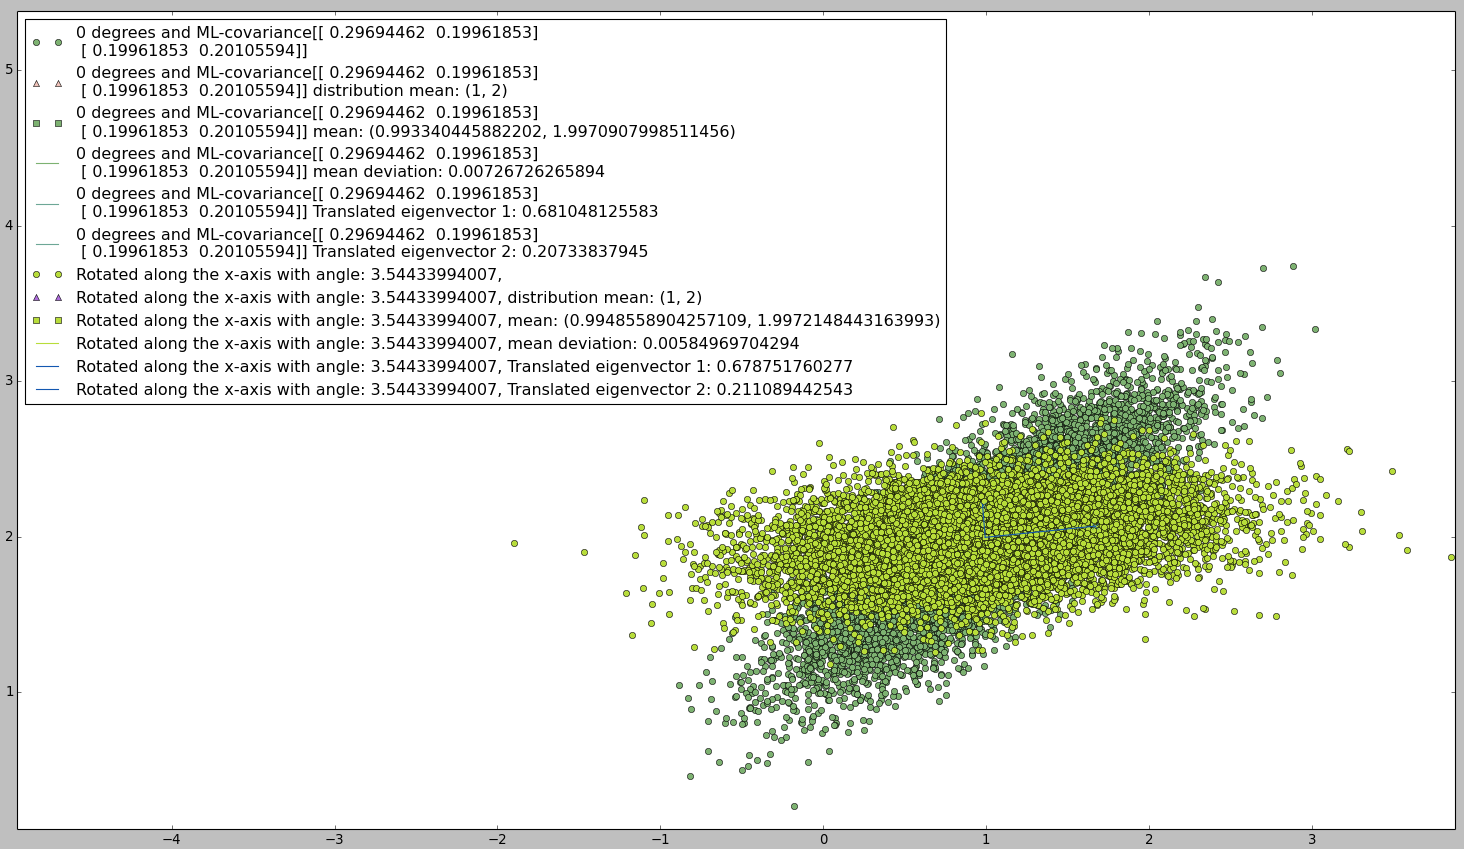
\includegraphics[width=\textwidth]{7.png}

\end{itemize}

\section{I.3.1}

Running the algorithms for various k's, we get the following accuracies:

\begin{itemize}
\item[-] k = 1; 0.815789473684\%
\item[-] k = 3; 0.710526315789\% 
\item[-] k = 5; 0.736842105263\%
\end{itemize}

As such, k = 1 is clearly the best k for this training- and test set.

\section{I.3.2}
\begin{itemize}
\item \textit{A short description of how you proceeded (e.g., did the
cross-validation)}

Initially the algorithm creates $S$ pairs of test and training sets .

Then it iterates through each value of $k$ (up to $k_{max}$) and calculates the accuracy for each test/training pair, by giving the data-points from the test set, to the nearest\_neightbour-function, that is trained with the corresponding training set.

If the accuracy is greater then the previous $k_{best}$, then this will be the new $k_{best}$

The program then returns the $k_{best}$.

\item \textit{Number of neighbors as suggested by hyperparameter selection}

When run, the program suggests $k_{best} = 3$.

\item \textit{Training and test error of $k_{best}$-NN}

This yields an accuracy $0.710526315789$\% for the test set, using $k_{best} = 3$. This is the same as having an classification error equal to $1 - 0.710526315789 = 0.289473684$\%. 

\end{itemize}


\section{I.3.3}
\begin{itemize}
\item \textit{Mean and variance of the training data}

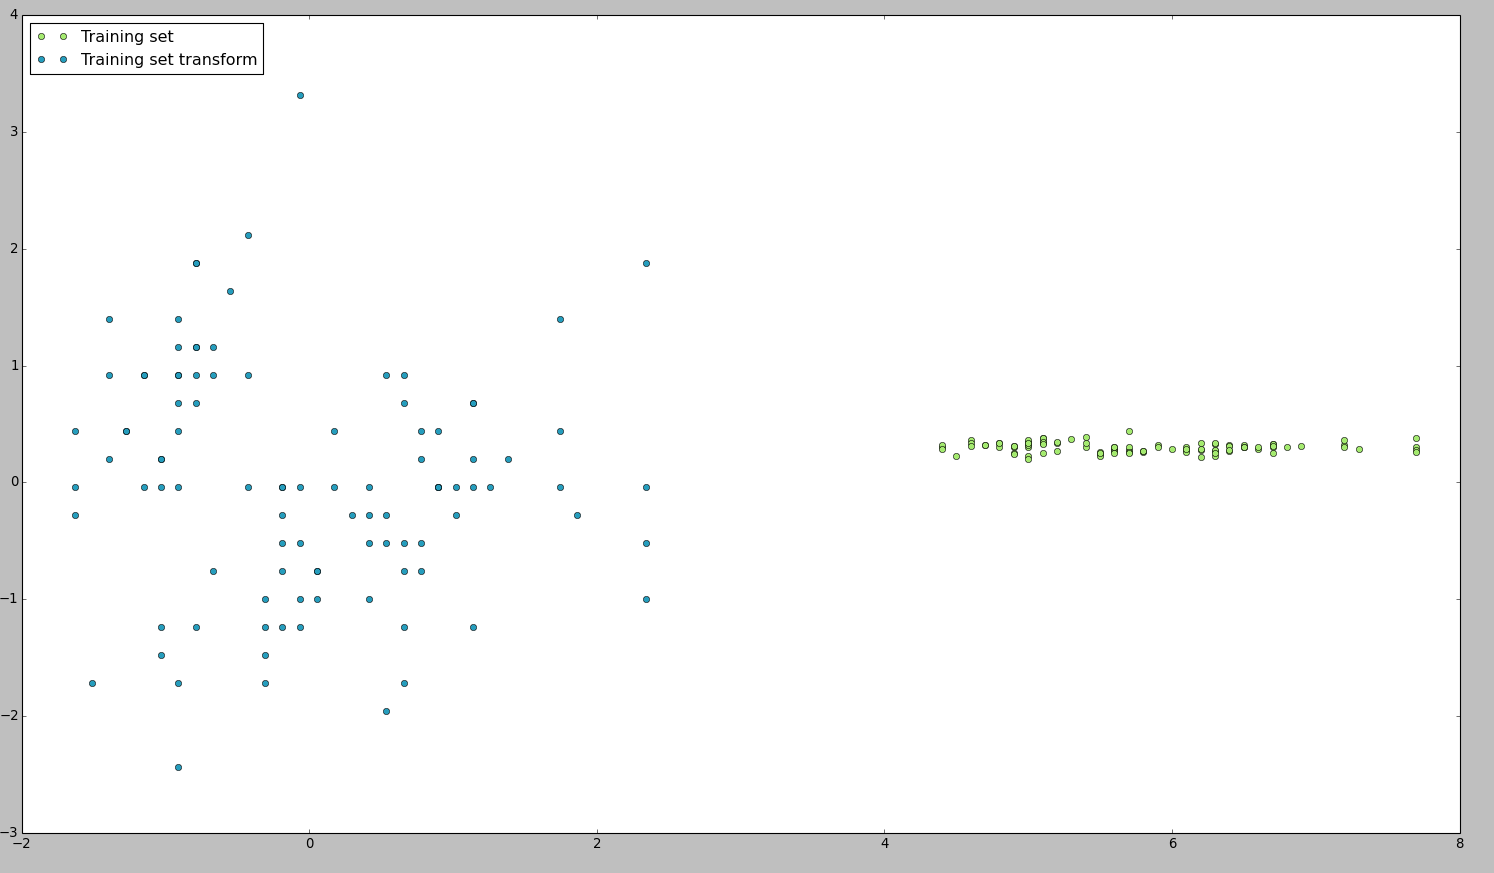
\includegraphics[width=\textwidth]{8.png}

We calculate the mean and variance of all N dimensions. In this case, our means are as follows:

Dimension x mean: 5.7560000000000029 \\
Dimension y mean: 0.30170000000000002

Dimension x variance: 0.8299783129696825 \\
Dimension y variance: 0.041738591255575462

\item \textit{mean and variance of the transformed test data}

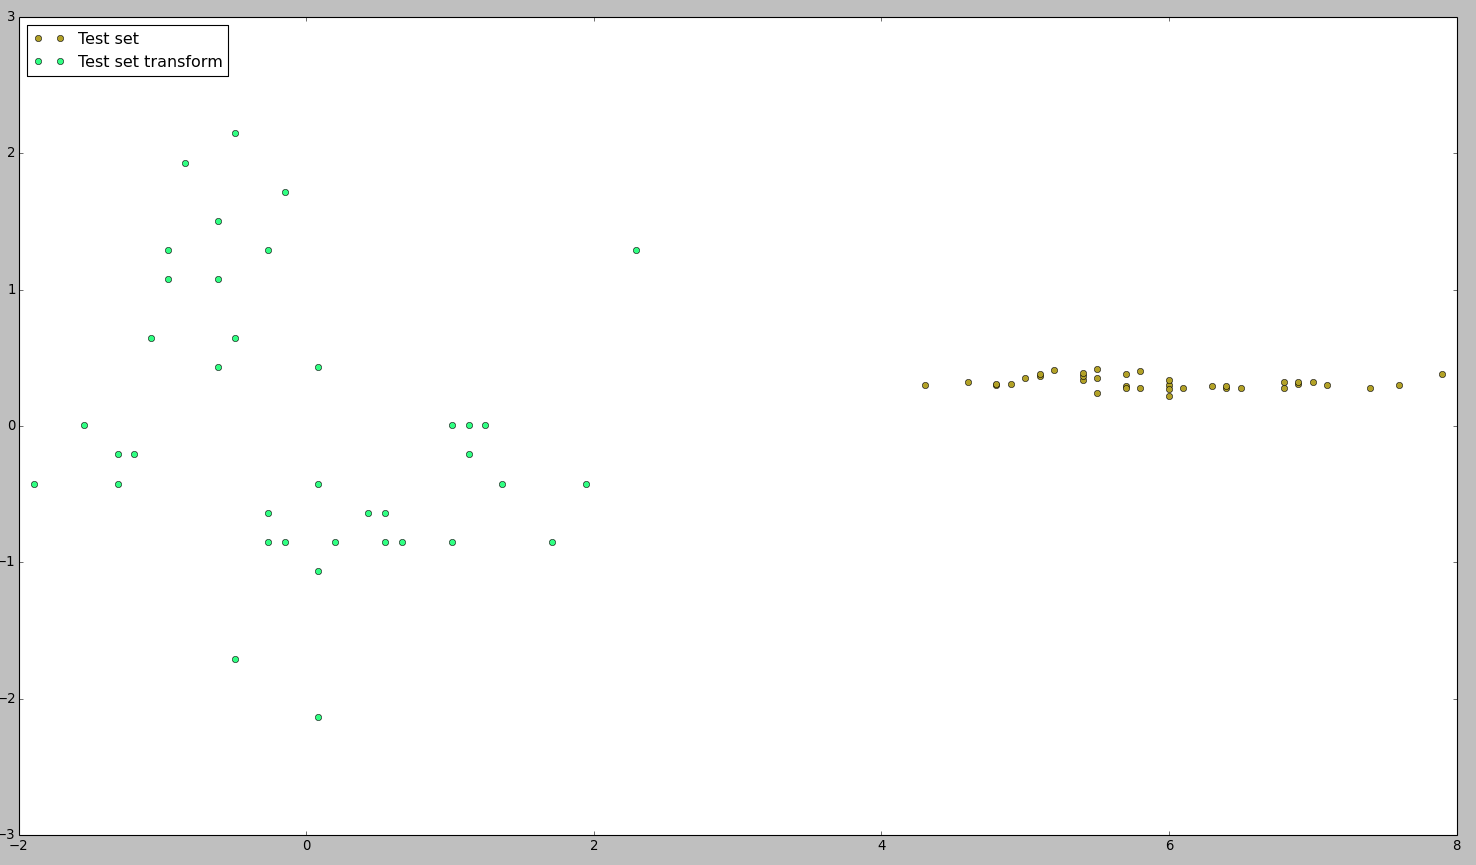
\includegraphics[width=\textwidth]{9.png}

Dimension x mean: 1.4316033738587545e-16 (Practically 0) \\
Dimension y mean: 1.4316033738587545e-16 (Practically 0)

Dimension x variance: 1.0 \\
Dimension y variance: 1.0

\item \textit{$k_{best}$ as suggested by cross-validation}

Running our cross-validator function on the normalized training set, we get $k_{best}$ to be $7$.

\item \textit{Can you explain the differences compared to the results achieved using the raw (not normalized) data?}

When we normalize across all axes (Dimensions), we essentially stretch the data points out to their normalized form, which normalizes the euclidean distances between all data points. This results in better results from the Nearest Neighbors algorithm, as we will now get less relative variance in the euclidean distances from our test data points to all the training data points.

\end{itemize}
\end{document}

